

% TESTING SETUP
% Solutution w SIP
% SIPML5 js library
% SIP traces
% webrtc2sip gateway
% 	installation
% 	configuration
% 	test

% ANALYSIS
% software used
% 	chrome/firefox nightly
% 	wireshark
% 	sip softphones
% webrtc w html5 socket
% using webrtc2sip gateway for sipows to sip conversation
% wireshark logs + browser console, call flows, media flows, code snippets, screenshots, SIP traces and architecture diagrams

Testing serves to validate that the suggested interworking components mentioned in the previous chapter accomplish their intended aim. This is to show that the gateway model suggested works.

\section{Testing objective}
Since developing a \gls{wrtc} gateway is a huge amount of work, beacuse of all the protocols and security measures that have to be implemented, I will not actually create a gateway in this thesis. However, I will use an open-source WebRTC gateway that uses SIP as its signaling protocol. Since SIP is pretty much the industry standard for doing signaling in the telecommunications industry, I see this as a good approach for testing purposes. This part will first start by introducing the libraries used for testing. Then I will give a quick overview of the testing environment. Lastly I will analyze a few calls to see what's going on during the interaction.

\section{Testing setup}
The experiments in this chapter are done using sipml5\footnote{http://sipml5.org/}, which is an open-source HTML5 SIP client using WebRTC for the media stack (natively provided by the browser). It uses SIP and SDP stacks written in javascript over WebSockets for signaling. For interoperability with native SIP clients it uses the webrtc2sip\footnote{Smart SIP and Media Gateway to connect WebRTC endpoints} gateway to act as a SIP proxy for translating the signaling. This gateway also includes a RTCWeb Breaker to convert the media streams and a Media Coder for transcoding. It operates very similar to my proposed architecture. In addition it connects to any SIP endpoint directly from the browser. The web browser used for testing is Google's Chrome (Version 34). A range of different SIP softphones is used as seen in Table \ref{tbl:sip-client-webrtc-interaction}. Wireshark\footnote{Wireshark is a network protocol analyzer} is used for traffic analysis in addition to Chrome Developer Tools\footnote{The Chrome Developer Tools are a set of web authoring and debugging tools built into Google Chrome}.

\section{Analysis}
I will break down each component of the gateway and test the interaction between client endpoints during a call session.

\subsection{The Signaling proxy}
In the signaling component a proxy solution was proposed to use a SIP stack for Javascript running over WebSockets. Using sipml5 and a range of different desktop SIP clients I tested to see how well the SIP proxy worked.  

\begin{table}[h]
\resizebox{\textwidth}{!}{%
\begin{tabular}{|p{1.3cm}|l|l|p{4cm}|p{4cm}|p{5cm}|}
\hline
SIP desktop clients & Audio & Video  & Latency                                                                                         & Quality                                                  & Comments                                                                                                            \\ \hline
Ekiga               & g.711 & failed & none                                                                                            & good audio quality                                       & did not get video working                                                                                           \\ \hline
Zoiper              & g.711 & vp8    & none for audio, video took approximately 5 seconds to appear, but then it was a live connection & good audio quality, huge packet loss on the video stream & good audio quality, but poor video quality conference                                                            \\ \hline
Jitsi               & g.711 & failed & none                                                                                            & good audio quality                                       & connection failed every time the application tried to negotiate a video codec, but worked fine when disabling video \\ \hline
Blink               & opus  & failed & none                                                                                            & good audio quality                                       & did not get video working                                                                                           \\ \hline
\end{tabular}
}
\caption{SIP desktop client interaction with web client using proxy and RTCWEB}
\label{tbl:sip-client-webrtc-interaction}
\end{table}

In figure \ref{tbl:sip-client-webrtc-interaction} the audio and video columns refer to the mutually agreed upon codec to be used during the signaling process. Since g.711 is the most preferred codec to be used in \gls{voip} systems, it is natural that audio most often defaults to this codec. Experiments with video conferencing was not very successful, it was difficult getting a normal video session to work for various reasons, one of them being a mismatch in the \gls{sdp} which was noted in the previous chapter as a probable outcome. The one desktop client that did manage to get a working video session using the VP8 codec had a very high packet loss as seen in figure \ref{fig:wireshark-sip-call}. Reasons for this is hard to say as the experiment was done on a really good connection.

\begin{figure}[here]
\centerline{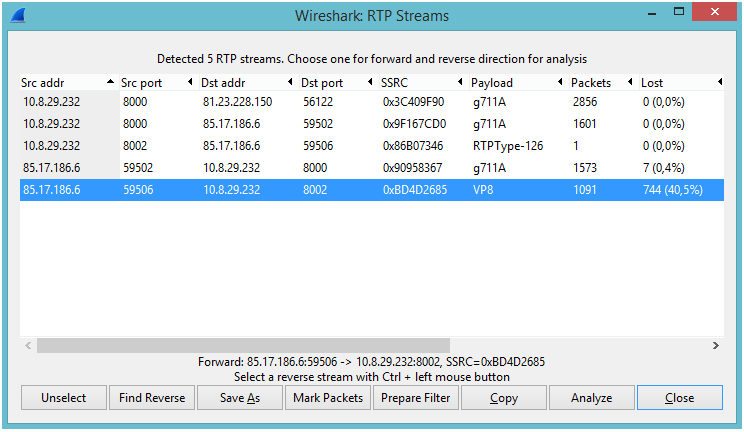
\includegraphics[scale=0.6]{wireshark-rtp.png}}
\caption{Wireshark analysis of a SIP call}
\label{fig:wireshark-sip-call}
\end{figure}

\subsection{The Transport Proxy}
Not much problems here, the connections were smooth with low latency, even running behind a proxy the connection felt `live'. The RTCWeb Breaker seems to work exactly as it should. As mentioned earlier there was no problems doing audio calls, but video calling seemed to cause some problems, this is probably not related to this component, since audio runs over the same protocols as video. It is probably to do with the clients not being able to agree on a common video codec. In Figure \ref{fig:wireshark-sip-call-flow} we can see an anlysis of the SIP call flow. We can see the call setup and the codecs which were offered. The codecs used in this case was the g.711 codec for audio. Lastly there is an acknowledgement of the hang up.

\begin{figure}[here]
\centerline{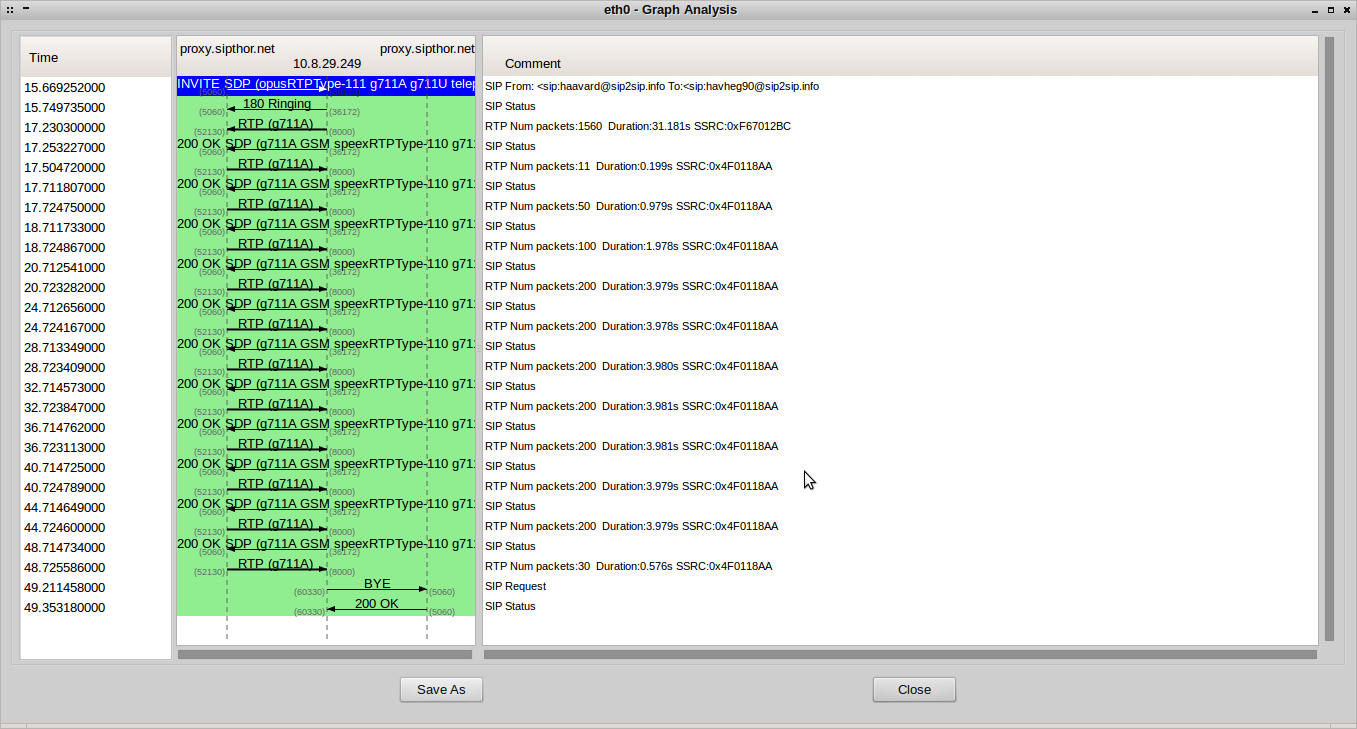
\includegraphics[scale=0.25]{call-flow.png}}
\caption{Wireshark SIP call flow}
\label{fig:wireshark-sip-call-flow}
\end{figure}

\subsection{The Media Transcoder}
\begin{quote}
Please note that the Media Coder will most likely be disabled on the sipml5.org hosted server. - http://sipml5.org/expert.htm
\end{quote}
There was not an agreement on which codec to use in the Web->Jitsi experiment. Jitsi only supports the H.264 video codec and Chrome the VP8 codec. It seems the media transcoder did not kick in, otherwise it probably could have worked. For the other cases, I'm not sure why video won't work, but I'm guessing there is a mismatch in the \gls{sdp}. Since transcoding can be done in the cloud, the quality should not really be affected by this component. With todays hardware we can do live-transcoding. Which codec used can somewhat limit latency, but the biggest latency issue has to do with the clients physical geographic location. The closer a client is to the media server the better, as the media doesn't have to travel that far.

\section{Summary}
By testing the open-source webrtc2sip gateway I show that developing a gateway for WebRTC is possible. The reason for the poor video quality could be several places, but I believe that because the connection had to go through a proxy for delivering the media, this is probably the cause. The next chapter will dive deeper into what it takes to build a gateway for an enterprise communication system. 




